\chapter{Theory of Operation} % How it should work in theory
\labch{tc-theory-of-operation}

The tesla coil was invented by Nikola Tesla in 1891. His vision was to use this technology to wirelessly transmit power to people all over the world. While his plans didn't meet the expectations by far, he still opened up a whole new field of physics, which today helps power the modern world.

Tesla coils come in a huge variety of sizes, power and modes of operation. From simple spark gap tesla coils, which consist of only a few passive components, to solid state tesla coils, whose only limitations are one's technical skills, every single one amazes anew by combining the world of High Voltage and High Frequency.

In order to understand the class E topology which this thesis is about, we have to understand the basics first. 

\section{The Tesla Resonator}

A tesla resonator, also called tesla coil, is a resonant transformer consisting of two loosely coupled air-cored windings: the primary and secondary coil. The primary coil, hooked up to the driver circuit on one side and grounded on the other, is usually made out of every few turns of thick wire. It is placed around the bottom of the secondary coil, either shaped like an flat spiral, a concentric cylinder, or at any angle in between. The secondary coil on the other hand has a lot more turns and is a lot higher.

\begin{marginfigure}[*-5]
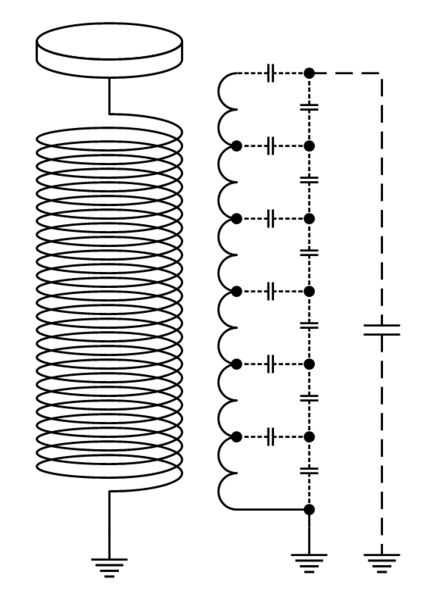
\includegraphics[width=\textwidth]{simon/resources/teslaCoilStrayCapacitance.png}
\caption{Stray capacitances of the secondary coil}
\labfig{teslaCoilStrayCapacintance}
\end{marginfigure}

As every real component, a coil has parasitic effects. The one relevant to a tesla coil's operation is the parasitic capacitance. A capacitance is just two different isolated voltage potentials, which is exactly, what we have along every single winding of a coil. This makes clear that every coil is actually an LC oscillator. The lower the inductance and capacitance of the coil, the higher the resonant frequency. This means that in order to lower the frequency to the desired one, many tesla coils have a top load, which, amongst others, acts like as an additional capacity towards ground.

If a high voltage, whose frequency is the resonant frequency of the secondary, is now applied to the primary coil, the LC circuit in the secondary coil starts oscillating and a very high voltage builds up gradually. Depending on the size and power of the tesla coil, this voltage can range from a few thousand to a few million volts. Once the voltage is high enough to ionise the air around the top\sidenote{This usually happens at a designated spark point}, it quickly discharges and the cycle starts over again.

\section{Exciting The Resonator}

There are various circuits which can be used for the excitation of the coil. Depending on the desired spark length, size\sidenote{The size of the secondary coil mostly determines its resonant frequency}, sensitivity to external effects, noise level and efficiency, different tesla coil drivers can be used. While Tesla's coils all used a spark gap topology, today we are able to use solid state devices to control the coil instead.

\subsection{The Spark Gap Tesla Coil}

\begin{marginfigure}
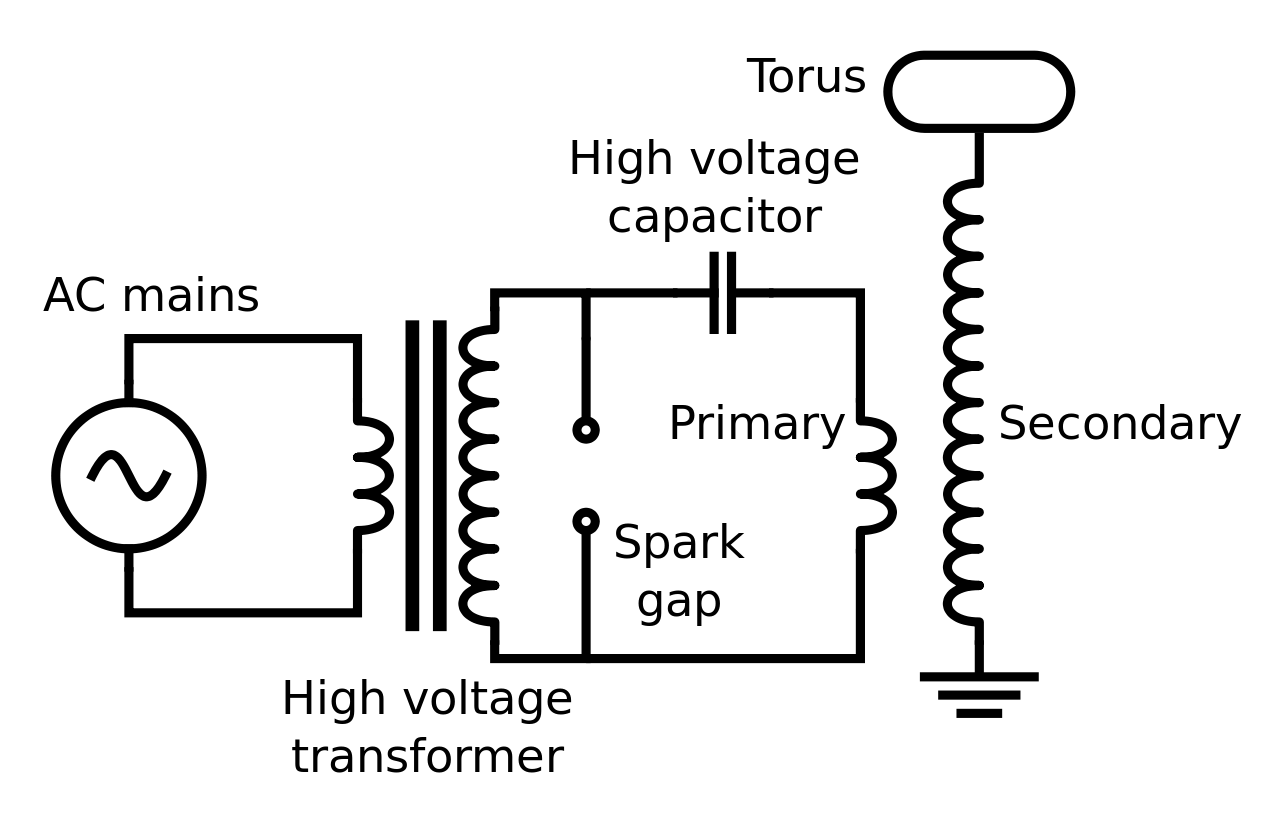
\includegraphics[width=\textwidth]{simon/resources/sparkGapTeslaCoil.png}
\caption{A simple spark gap tesla coil}
\labfig{sparkGapTeslaCoil}
\end{marginfigure}

The simplest and oldest of all drivers is the spark gap driver. In the first stage, the 230V mains voltage is transformed to a few kilovolts. Neon sign or microwave transformers are popular choices for this task. The capacitor gets charged up until the voltage is high enough to break through the spark gap. The spark gap then has a very low resistance and allows the current to oscillate between the capacitor and the primary coil. This oscillation frequency is usually in the order of ten to hundred kilohertz and is the same frequency as the resonant frequency of the secondary coil. In every cycle, a little energy is transferred to the secondary via the magnetic coupling of the coils. When the voltage in the secondary gets too high, a breakout occurs. This can happen one or more times within a period of the AC mains voltage. Once all the energy in the primary circuit has been transferred to the secondary or dissipated as heat, the spark gap \enquote{quenches} allowing the capacitor to charge up again.

Today, spark gap tesla coils are mostly only used for educational purposes anymore. Due to their many \textbf{disadvantages} they are avoided when power efficiency and noise level play a role. The disadvantages most worth mentioning include:

\begin{itemize}
\item A spark gap dissipates a lot of power, part of it as heat and part of it in creating a ozone, which also poses a health hazard, when operated in closed rooms.
\item The rapid igniting and quenching of the spark gap creates a lot of noise.
\item The whole operation cycle only depends on passive component values, which makes it very hard to control the power output and other characteristics.
\end{itemize}

\subsection{Solid State Tesla Coils}

Aside from vacuum tube tesla coils, which have existed before, semiconductor technology\sidenote{Unlike relays or hard disk drives, their semiconductor counterparts have no moving components. Hence the name \enquote{solid state}.} opened up a whole new world of possibilities for tesla coils. It was now possible to build up sophisticated amplifier circuits to excite the primary coil. Some of them still rely on resonant circuits, others use feedback loops to self-excite the primary coil, and again others use \glspl{ic} to control the driver.

The most common solid state topologies include:
\begin{itemize}
\item Slayer exciter
\item Half-bridge / full-bridge (single or dual resonant)
\item Class E
\end{itemize}

\subsubsection{Slayer Exciter Circuit}

The slayer exciter topology is the most common under hobbyist coilers\sidenote{This is how people building tesla coils often call themselves}, because it's by far the simplest one, only consisting of very few components. At it's hard sits the Transistor T controlling the current through the primary coil L1. When first powering on the circuit, current flows through R into the base of T, allowing current to flow through L1, creating a magnetic field.\sidenote{Since the magnetic field flows through both coils in the same direction, the winding direction of the secondary has to be reversed so that the output voltage won't be reversed.} The rapid change in the field induces a high voltage in the secondary coil L2. The parasitic capacitance C of L2 however only lets the voltage across it rise slowly, therefore pushing the potential of the bottom of the lower end of L2 to a negative voltage. As soon as the voltage falls below -0.7V, the diode D starts conducting and limits the negative voltage while providing current to charge up C\sidenote{The diode could be left out, since the base emitter junction also acts as diode, but in the most cases this damages the transistor}. Additionally, since the base emitter voltage is now negative, T stops conducting. This causes the magnetic field to start collapsing, causing the potential at the base to slowly rise, until T starts conducting again. The circuit is now in it's initial state, except that C is now charged to a high voltage and the process starts over again.

Since the timing of the circuit only depends on the values of L1, L2, and C, the circuit tunes itself, which makes it very stable to operate. But because of its simplicity it comes with a few disadvantages. Firstly, when T is conducting, it basically shorts L1, which leads to a high current and therefore power dissipated in T. This power can be reduced by choosing R to be rather high. This reduces the base current and therefore also the collector current. While this helps reducing the power dissipation it also reduces the output power of the coil. With a bit of extra complexity this circuit can however be made more efficient.

\begin{figure}[h!]
\centering
\begin{circuitikz}[european, american inductors]
  \draw (2,4) to[short, *-] (0,4) to[battery, l=V] (0,0) node[ground]{};
  \draw (2,4) to[R, l=R] (2,1) to[D-, l=D] (2,0) node[ground]{};
  \draw (4,1.5) node[npn](npn){T};
  \draw (2,4) -- (4,4) to[L, l_=L\textsubscript{1}] (npn.C);
  \draw (npn.C) ++(-.2,.4) node[circ]{};
  \draw (npn.E) -- (4,0) node[ground]{};
  \draw (npn.B) to[short, -*] (2,1.5);
  \ctikzset{inductors/coils=10, inductors/width=2}
  \draw (5,.5) to[L, l=L\textsubscript{2}] (5,4) -- (6,4) to[C, l=C] (6,0) node[ground]{};
  \draw (5,4) ++(.2,-.4) node[circ]{};
  \draw (3,1.5) to[short, *-] (3,.5) to[crossing] (5,.5);
\end{circuitikz}
\caption{Slayer exciter circuit}
\end{figure}

\subsubsection{Half-Bridge / Full-Bridge}

This design drives the primary coil by a half or full bridge. While this requires large and expensive power MOSFETs or IGBTs as well as carefully designed GDTs\sidenote{Gate drive transformer}, it offers a lot of flexibility and power up to many kW.

\begin{figure}
\captionsetup[subfigure]{labelformat=empty}
\centering
\begin{subfigure}{.5\textwidth}
  \centering
  \begin{circuitikz}[european, american inductors]
  \draw (0,0) node[nigfete](n2){};
  \draw (n2.S) node[tlground](g1){};
  \draw (0,2) node[nigfete](n1){};
  \draw (n1.S) -- (n2.D);
  \draw (0,1) node[circ]{} to[L] (2,1) node[circ]{};
  \draw (g1 -| 2,2) node[tlground]{} to[C] (2,1) to[C] (n1.D -| 2,1) -- ++(-2,0);
  \draw (n1.D -| 1,2) node[vcc]{};
  \end{circuitikz}
  \caption{Half bridge design}
\end{subfigure}%
\begin{subfigure}{.5\textwidth}
  \centering
  \begin{circuitikz}[european, american inductors]
  \draw (0,0) node[nigfete](n2){};
  \draw (n2.S) node[tlground](g1){};
  \draw (0,2) node[nigfete](n1){};
  \draw (n1.S) -- (n2.D);
  \draw (0,1) node[circ]{} to[L] (2,1) node[circ]{};
  \draw (2,0) node[nigfete, xscale=-1](n4){};
  \draw (2,2) node[nigfete, xscale=-1](n3){};
  \draw (n3.S) -- (n4.D);
  \draw (n4.S) node[tlground]{};
  \draw (n1.D -| 1,2) node[vcc]{};
  \draw (n3.D) -- (n1.D);
  \end{circuitikz}
  \caption{Full bridge design}
\end{subfigure}
\end{figure}

The decision between a half bridge or full bridge design is a tradeoff between the number of parts and the output power. Due to the two capacitors in the half bridge design, the second end of the primary coil is biased at  \(\nicefrac{V_{CC}}{2}\), which means that the maximum voltage across the primary coil can also be only \(\nicefrac{V_{CC}}{2}\). However, a working half bridge design can rather easily be expanded to a full bridge design, which can then utilize the whole supply voltage.

A half or full bridge design can be deployed either single or dual resonant\sidenote{Mostly known as Dual Resonant SSTC or DRSSTC}. In order to turn a single resonant design into a double resonant design, a capacitor is added to the primary circuit which turns it into an resonator with the same resonant frequency as the secondary coil. Since the reactance of an LC circuit is the lowest at its resonant frequency, it draws a lot more current than the primary coil alone, resulting in more power transmitted to the secondary coil.

This design is often used for medium-sized to large tesla coils due to its high output power. However, due to the MOSFETs\sidenote{Or other switching devices, like IGBTs} switching a high current at a high voltage, a lot of power is dissipated and they have to be adequately cooled. The stress on the MOSFETs can be reduced a bit by interrupting\sidenote{Turning the coil off and on very quickly} the tesla coil. Additionally, this allows the plasma channels to quench during each interrupting cycle, raising its resistance and therefore the breakout voltage, which in turn raises the length of the arcs. So this technique lowers the stress on the switching devices, lowers the input power and raises the arc length. The only drawback is that the arcs sound a lot harsher and louder.

A big advantage of the bridge design is, that unless a dual resonant design is chosen, the switching frequency is only determined by the circuit driving the bridge. This allows it to work across a very wide range of frequencies and even follow the slightly changing resonant frequency of the secondary coil in real time.

\subsubsection{Class E}

This topology uses a class E amplifier to produce the necessary power for driving the primary coil. By utilizing a technique called \gls{zvs} and \gls{zcs}, the dissipated power in the switching device can be drastically reduced, making this type of amplifier nearly 100\% efficient in theory. A class E amplifier is capable of switching very high frequencies, which makes it an ideal driver for smaller tesla coils operating at and above a few MHz.\sidenote{Other conventional power amplifiers are also able to switch such high frequencies, but they need special and very costly power semiconductors.}

\section{Class E Amplifier}

The problem with conventional class B or C amplifiers is that with increasing switching speed, the efficiency drastically falls. This is because the turn-on and turn-off times become an increasingly large part of the total period with higher frequencies. While the MOSFET transitions from low to high resistance or vice versa, it dissipates a lot of power, when a voltage is applied. By ensuring that the voltage across the switching device is zero during turn-off and turn-on, the class E amplifier aims to solve this problem.

\subsection{Theory of Operation}

The goal of the class E amplifier is to reach very high efficiencies for frequencies upwards of a few MHz, and by minimizing its power dissipation. Power dissipation is the product of voltages times current, so the easiest way to minimize it is to keep either voltage or current close to zero at all times. Typically simultaneous high current and voltage occur during the switching period, when the switching device has (in theory) non-zero, finite resistance. Therefore this kind of amplifier utilizes a reactive load network, which forces the voltage across the switching device to zero just before turn-on and the current to zero just before turn-off.\sidenote{This technique is commonly called \gls{zvs} / \gls{zcs}.} This also means, that the switching device is no longer used as an amplifier, but rather as a switch\sidenote{This type of amplifier is often referred to as switching mode amplifier} and the load network then shapes the output voltage. Figure \ref{fig:class-e-basic} shows the basic class E amplifier and figure \ref{fig:nominal-waveforms} its nominal voltage across and current through a real MOSFET.

\begin{figure}[h!]
  \centering
\begin{circuitikz}
  \draw (0,0) node[nigfete](nmos){};
  \ctikzset{capacitors/width=0.075, capacitors/height=0.25}
  \draw[dashed] ([yshift=-7] nmos.D) -- ++(.35,0) -- ++(0,-.35) node(c1){};
  \draw (c1) to[C] ++(0,-.35);
  \draw[dashed] (c1) ++(0,-.35) -- ([yshift=7] c1 |- nmos.S) to[short] ++(-.35,0);
  \ctikzset{capacitors/width=0.1, capacitors/height=0.4}
  \draw (nmos.S) node[rground]{};
  \draw (nmos.D) to[cute choke, twolineschoke, l_=L\textsubscript{1}] ++(0,2) node[vcc]{};
  \draw (nmos.D) ++(0,.2) to[short,*-] ++(1.5,0) to[C, l=C\textsubscript{1}] ++(0,-1.75) node[rground]{};
  \ctikzset{resistors/scale=.8}
  \draw (nmos.D) ++(1.5,.2) to[short,*-] ++(.5,0) to[L, l=L\textsubscript{2}] ++(1,0) to[C, l=C\textsubscript{2}] ++(1,0) -| ++(.5,-.3) to[R, european, l=R\textsubscript{L}] ++(0,-1.45) node[rground]{};
  \draw[dashed, gray] (nmos.D) ++(-.7,1.75) -- ++(1.5,0) -- ++(0,-.75) node[above right]{Load network} -- ++(3.25,0) -- ++(0,-1.25) -| ++(-1.6,-.8) -| ++(-1.5,1.4) -| ++(-1.65,1.4);
\end{circuitikz}
  \caption{Class-E amplifier}
  \label{fig:class-e-basic}
\end{figure}

\begin{figure}[h!]
    \centering
    \begin{tikzpicture}
    \begin{axis}[
      grid=both,
      ticks=none,
      ]
      \addplot table [x=x,y=y,col sep=comma, mark=none] {simon/resources/nominal_voltage.csv};
      \addlegendentry{Voltage};
      \addplot table [x=x,y=y,col sep=comma, mark=none, smooth] {simon/resources/nominal_current.csv};
      \addlegendentry{Current};
    \end{axis}
    \draw (0,0) rectangle (3.432,-.25);
    \node at (1.78,-.125) {\tiny OFF};
    \draw (3.435,0) rectangle (6.855,-.25);
    \node at (5.34,-.125) {\tiny ON};
    \end{tikzpicture}
    \caption{Nominal Class-E waveforms}
    \label{fig:nominal-waveforms}
\end{figure}

One big problem with this type of amplifier however, is that the voltage and current quickly exceed the safe operating range of the switching device. The voltage can get up to four times the supply voltage and the current up to three times the supply current. This is however highly dependent on the used duty cycle, which should also be taken into consideration, when designing such an amplifier. However, because this would add a lot of complexity to both the design process and the driver circuit, the duty cycle was defined to be 50\%.


\subsection{The Class-E Amplifier as Tesla Coil Driver}

\section{Musical Tesla Coils}

Musical Tesla coils have been getting a lot of attraction since the mid-2000s and are probably the reason for the popularity of tesla coils in general. To many it's simply mind-blowing how a single arc can produce anything musical. But the physics behind it is in fact very similar to that of a conventional speaker using a membrane.

In a tesla coil's usual, uninterrupted operation mode, the high voltage in the secondary coil causes a plasma channel (the arc) to form, discharging the coil. Since the plasma takes up a much higher volume, it expands rapidly and pushes air away from the coil. Once discharged, the plasma channel extinguishes and the secondary coil begins to charge up again. A single discharge creates a \enquote{snapping} sound well known from arcs, but in a tesla coil this cycle repeats many times a second, resulting in a harsh, square-wave-like sound. Mostly depending on the size of the coil, this frequency can be a few hundred hertz to tens of kilohertz; some smaller coils even exceed the human-audible range, creating a noiseless flame-like discharge.

By modulating another frequency onto this carrier frequency, a.k.a. turning the coil on and off at this rate, the frequency is also modulated onto the sound wave created by the arcs. Since the tesla coil has to complete at least one cycle before being turned off, the modulated frequency cannot be greater than the carrier frequency. 

Figure \ref{fig:arcing-activity} shows the arcing activity\todo{find better word} of the tesla coil for the example of a 500 Hz signal modulated onto a 10 kHz carrier wave. Figure \ref{fig:sound-pressure} visualizes the movement of the air molecules around the tesla coil\sidenote{This graph is very likely not accurate and only indented for demonstration purposes}. By performing a Fourier analysis on figure \ref{fig:sound-pressure}, a graph of all frequency components of the sound wave can be created as shown in figure \ref{fig:frequency-magnitude}. It is clearly visible, that not only the modulated signal, but also the carrier frequency is audible, which distorts the sound. A method to counteract this is by using smaller tesla coils, which often have carrier frequencies well above the human hearing range.

\begin{figure}[h!]
\begin{tikzpicture}
  \begin{axis}[
    xmin=0,
    xmax=3.75,
    ymax = 1.2,
    ytick = none,
    xtick distance = 1,
    width = \textwidth,
    height = 5cm,
    axis y line = left,
    axis x line = middle,
    xlabel = \(t\) in \(ms\),
    %ylabel = arcing activity,
    scaled ticks = false,
    tick align = inside,
    x filter/.code=\pgfmathparse{#1 * 1000},
    area style,
    ]
    \addplot+[draw=black, fill=gr10] table [x=t, y=rect, col sep=comma, mark=none]{simon/resources/signal.csv};
    %\node at (02.5,112) {\resizebox{1.3mm}{!}{
\includegraphics{simon/resources/lighting.png}}};
    \node at (12.5,112) {\resizebox{1.3mm}{!}{
\includegraphics{simon/resources/lighting.png}}};
    \node at (22.5,112) {\resizebox{1.3mm}{!}{
\includegraphics{simon/resources/lighting.png}}};
    \node at (32.5,112) {\resizebox{1.3mm}{!}{
\includegraphics{simon/resources/lighting.png}}};
    \node at (42.5,112) {\resizebox{1.3mm}{!}{
\includegraphics{simon/resources/lighting.png}}};
    \node at (52.5,112) {\resizebox{1.3mm}{!}{
\includegraphics{simon/resources/lighting.png}}};
    \node at (62.5,112) {\resizebox{1.3mm}{!}{
\includegraphics{simon/resources/lighting.png}}};
    \node at (72.5,112) {\resizebox{1.3mm}{!}{
\includegraphics{simon/resources/lighting.png}}};
    \node at (82.5,112) {\resizebox{1.3mm}{!}{
\includegraphics{simon/resources/lighting.png}}};
    \node at (92.5,112) {\resizebox{1.3mm}{!}{
\includegraphics{simon/resources/lighting.png}}};
  \end{axis}
\end{tikzpicture}
\caption{Arcing Activity}
\labfig{arcing-activity}
\end{figure}

\begin{figure}[h!]
\begin{tikzpicture}
  \begin{axis}[
    xmin=0,
    xmax=3.75,
    ytick = none,
    xtick distance = 1,
    width = \textwidth,
    height = 5cm,
    axis y line = left,
    axis x line = middle,
    xlabel = \(t\) in \(ms\),
    %ylabel = sound pressure,
    scaled ticks = false,
    x filter/.code=\pgfmathparse{#1 * 1000},
    area style,
    ]
    \addplot+[draw=black, fill=gr10] table [x=t, y=disp, col sep=comma, mark=none]{simon/resources/signal.csv};
  \end{axis}
\end{tikzpicture}
\caption{Sound Pressure}
\labfig{sound-pressure}
\end{figure}

\begin{figure}[h!]
\begin{tikzpicture}
  \begin{axis}[
    xmode = log,
    xmin = 300,
    xmax = 22000,
    ymax = 60,
    ytick = {0},
    yticklabels = \empty,
    xticklabels = \empty,
    extra x ticks = {500,1500,2500,10000},
    width = \textwidth,
    height = 5cm,
    axis y line = left,
    axis x line = middle,
    tick align = inside,
    log ticks with fixed point,
    % 1000 sep = {\,},
    xticklabel style={/pgf/number format/.cd,1000 sep = {\;},fixed},
    scaled ticks = false,
    xlabel = \(f\) in \(Hz\),
    %ylabel = magnitude
    ]
    \addplot+[ycomb, draw=black, mark options={gr40}] table [x=f, y=mag, col sep=comma]{simon/resources/fourier.csv};
  \end{axis}
\end{tikzpicture}
\caption{Frequency Magnitude}
\labfig{frequency-magnitude}
\end{figure}

\todo{Add section on how to play multiple tones}

a

\subsection{Analog modulation}

.
